\chapter{Conclusions \& Further Work}
\label{cha:future_work}
\epigraph{This chapter draws come conclusions from the practical as well as
  theoretical considerations that were made during this work. Additionally it
  provides an outlook on how the developed model could be improved with respect
  to prediction and computational performance.
}

\section{Conclusions}%
\label{sec:conclusions}

After a considerable amount of thought was put into the understanding of the
dynamical nature and ESN and recurrent neural networks in general we
successfully implemented a framework that is able to predict high-dimensional,
spatio-temporal, chaotic time series.  By solving the prediction problem we
have in turn managed to create a fairly general anomaly detection algorithm for
said chaotic systems, without assuming anything about their internal physical
nature.  The results of sections \ref{sec:res_mackey_glass_system} and
\ref{sec:res_kuroshio} show the algorithm in action on simulated data.
Anomalies in the Mackey-Glass system as well as in climate model output have
been successfully detected.  The only thing that has to be adjusted from one
dataset to the next are a few hyper-parameters, which can be found via Bayesian
Optimization.  However, if this is infeasible, they can also be set
approximately by hand by reasoning about the specific requirements of the given
problem.  Both the state size and the spectral radius of the ESN can be chosen
within narrow bounds by examining the requirements of the problem. The state
size should be at least as large as the period of the examined sequence and the
spectral radius must be large enough to capture its non-linearity.  However, to
achieve the best results the exact choices of hyper-parameters are best left to
algorithms such as Bayesian Optimization.  This reduces the amount of tweaking
that has to be done to apply the model to new datasets to a minimum.  In
addition, the application of the ESN to the prediction problem has lead to a
very cost efficient search algorithm.

The second goal of finding new physical behaviour in the available climate
model output remains to be achieved. It will require some house keeping in the
analysis part of the code, but all the necessary parts are in place. To judge
the scientific value of the potential anomalies that are to be found will
require and experienced oceanographer.

With this proof of concept we have shown that the concepts of machine learning
can be of much use in the field of oceanography and climate physics as a whole.
A wider application of the concepts from artificial intelligence and machine
learning promises to make the full potential of climate data exploitable in
completely new ways.


\section{Predictor Improvements}
With the rather basic setup of a single ESN cell as the prediction network,
there is still much room for improvement of the prediction model.  The most
obvious improvement would be to add a number of  convolutional layers in front
of the ESN cell. This could lead to significant improvements by leveraging the
power of convolutional filters that were described in
Sec.~\ref{sub:convolutional_neural_nets}.  Unfortunately, they would make the
use of an expensive GD algorithm for the weight optimization necessary.
By sacrificing the convolutional layer for a feedforward layer the GD
optimization could be avoided, because it is possible to construct untrained
feedforward layers in a similar fashion as the ESN has an untrained reservoir.
Networks that contain untrained feedforward layers are called \emph{extreme
learning machines} and were introduced by [\cite{huang2006}].  The combination of
the two concepts was introduced by [\cite{butcher2013}] and termed
\emph{reservoir with random static projections} (R$^2$SP).  This architecture
promises to solve the memory non-linearity tradeoff by separating non-linear
transformation and internal memory of the network and could thus be much more
powerful.

\begin{figure}
  \centering
  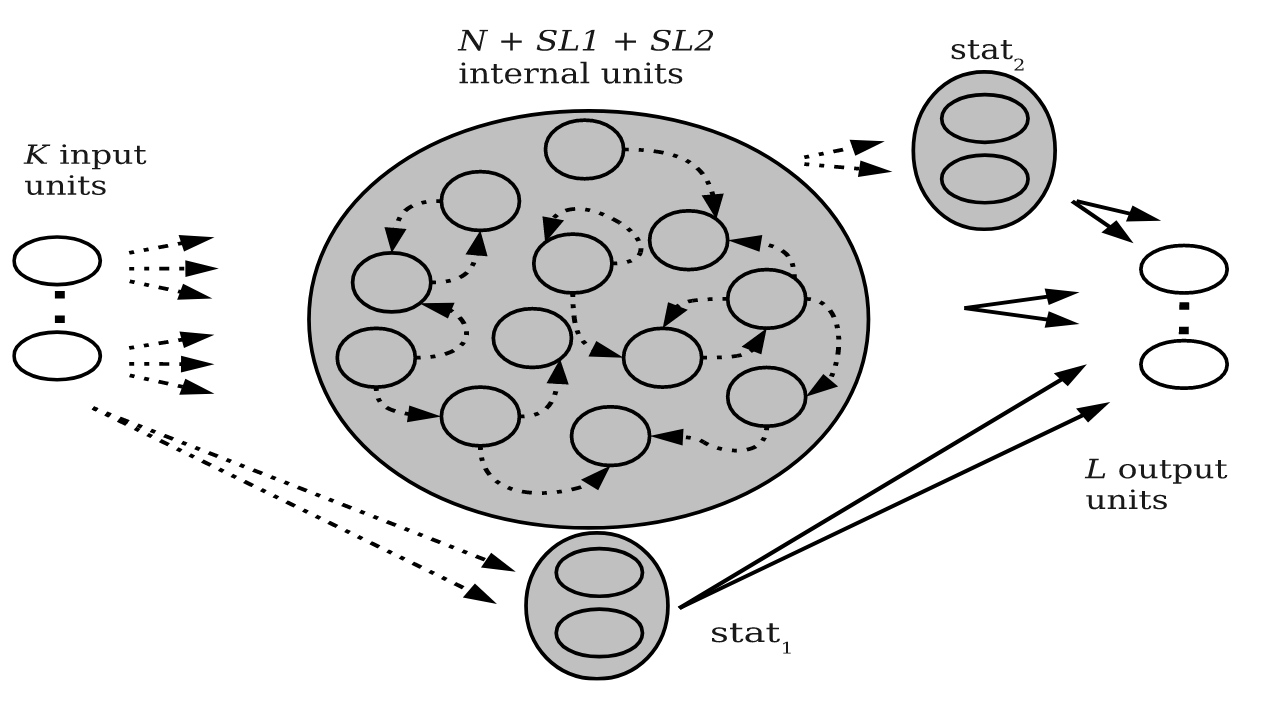
\includegraphics[width=0.6\linewidth]{r2sp.png}
  \caption{Reservoir with random static projections~[\cite{butcher2013}]. The
  stat$_1$ and stat$_2$ layers are static feedforward layers, that take the
  part of the non-linear transformation.  The recurrent internal units
  represent the memory of the network. Their reservoir matrix can be
  initialized with a spectral radius close to one to maximize memory without
  the need of introducing non-linearities.}
  \label{fig:r2sp}
\end{figure}

Another interesting approach to improve the performance of the network would be
to employ \emph{evolutionary optimization} techniques [\cite{fogel1997}] to find
good reservoir matrix $\wmatr{}$ which could be reused for the whole ocean
dataset.  This would eliminate fluctuations in prediction performance from run
to run.


\section{Performance Improvements}
Probably the greatest advantage of presented approach is its low computational
demand. Creating predictions of a few hundred frames for a window of 30x30 pixels
does not take longer than a few seconds on a standard laptop.
For a truly automated application of the model to very large datasets with long
sequences it would be interesting to implement it in another framework.
Tensorflow does not excel in RNN computations and it would be quite simple to
implement the network, for example, in Numpy and parallelize it with Bohrium
[\cite{bohrium}]. This would get rid of a lot of overhead that is caused by the
dynamic graph creation that Tensorflow is doing.

Additionally, the ESN, due to its static nature, holds the potential of being
compiled to an FPGA, which could improve performance even further.


\section{Understanding Recurrent Networks}

To date, the general understanding of the ESN and RNNs in general is not very
good.  It is assumed that an RNN classifier needs as many fixed points as it
has features to separate, but fundamental understanding is still lacking.  A
further investigation of the influence of fixed-points and period cycles within
the internal state evolution on the memory and predictive capabilities of RNNs
would be very interesting.  This could lead to a more solid understanding of
how the hyper-parameters of the ESN are influencing its performance.
